\documentclass{beamer}
\usepackage[utf8]{inputenc}
\usepackage{tikz}
\usepackage{verbatim}
\usetikzlibrary{arrows,shapes}


\usepackage{utopia} %font utopia imported

\usetheme{Boadilla}
\usecolortheme{default}

%------------------------------------------------------------
%This block of code defines the information to appear in the
%Title page
\title{Entrenamiento de modelos de aprendizaje profundo mediante autosupervisión}

\author
{Rubén Ezequiel Torti López}

\institute
{
  Facultad de Matemática, Astronomía, Física y Computación\\
  Universidad Nacional de Córdoba
}

\date
{Agosto 2017}

\logo{
\includegraphics[height=1.0cm]{images/UNC-footer.jpg}}

%End of title page configuration block
%------------------------------------------------------------





%------------------------------------------------------------
%gets rid of bottom navigation bars
\setbeamertemplate{footline}[frame number]{}

%gets rid of bottom navigation symbols
\setbeamertemplate{navigation symbols}{}

%gets rid of footer
%will override 'frame number' instruction above
%comment out to revert to previous/default definitions
\setbeamertemplate{footline}{}
%------------------------------------------------------------





%------------------------------------------------------------
%The next block of commands puts the table of contents at the 
%beginning of each section and highlights the current section:
%
%\AtBeginSection[]
%{
%  \begin{frame}
%    \frametitle{Table of Contents}
%    \tableofcontents[currentsection]
%  \end{frame}
%}
%------------------------------------------------------------




\begin{document}
%The next statement creates the title page.
\frame{\titlepage}
%---------------------------------------------------------
%This block of code is for the table of contents after
%the title page
%\begin{frame}
%\frametitle{Table of Contents}
%\tableofcontents
%\end{frame}
%---------------------------------------------------------




\section{intro}
%---------------------------------------------------------
\begin{frame}[plain]
\frametitle{Aprendizaje automático}
Explora algoritmos cuyo objetivo es identificar patrones en conjuntos de datos.\pause
\vfill

Supera el enfoque clásico de instrucciones estáticas, tomando decisiones basadas en datos.\pause
\vfill

Tareas demasiado complejas para programarse directamente:
\vfill
\begin{block}{Ejemplos}
\begin{itemize}
    \item Detección y verificación de caras
    \item Autos que se manejan solos 
    \item Reconocimiento del habla
    \item Diagnósticos médicos 
\end{itemize}
\end{block}
\end{frame}
%---------------------------------------------------------





%---------------------------------------------------------
\begin{frame}
\frametitle{Aprendizaje Supervisado - No Supervisado}
\begin{figure}
    \centering
    \begin{subfigure}
        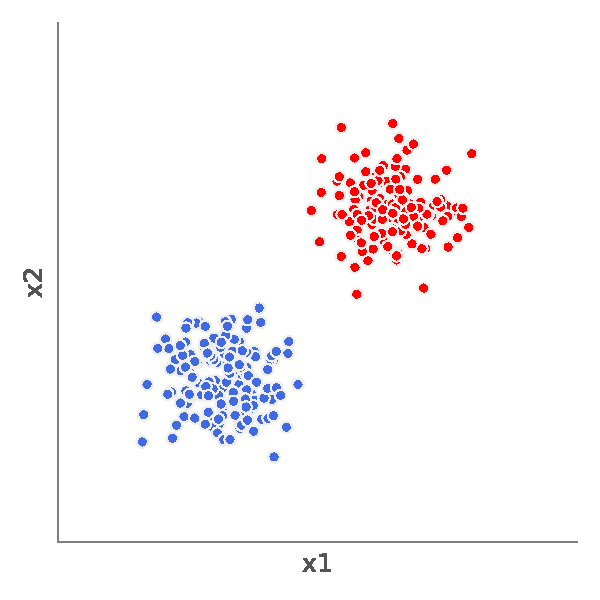
\includegraphics[width=0.4\textwidth]{images/machinelearning1.pdf}
    \end{subfigure}
\quad
    \begin{subfigure}
        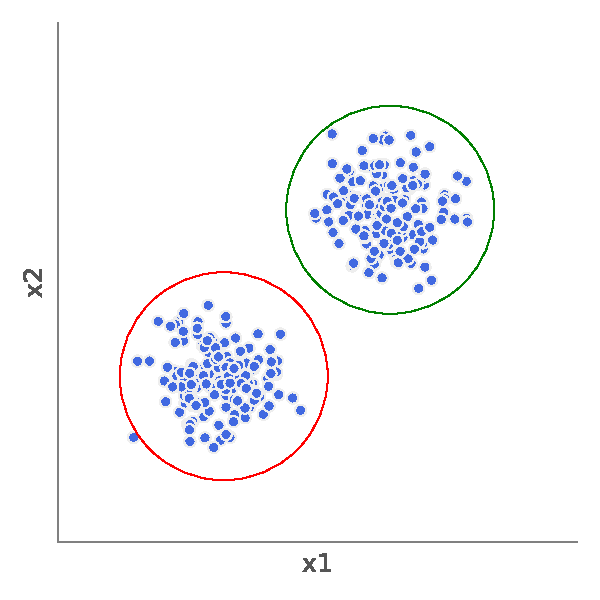
\includegraphics[width=0.4\textwidth]{images/machinelearning2.pdf}
    \end{subfigure}
\end{figure}
\end{frame}
%---------------------------------------------------------





\section{marco}
%---------------------------------------------------------
\begin{frame}[plain]
\frametitle{Visión por Computadoras}
Busca describir y reconstruir propiedades del entorno a partir de imágenes.\pause
\vfill
\textit{Problema inverso}.\pause
\vfill
Es necesario recurrir a modelos físicos y/o probabilísticos\pause
\vfill
\begin{figure}
    \centering
    \begin{subfigure}
        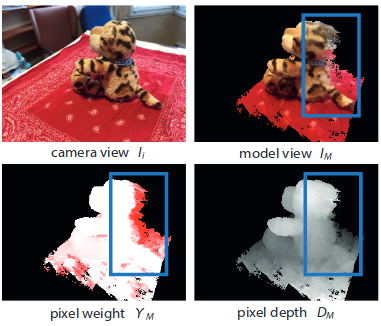
\includegraphics[width=0.3\textwidth]{images/computer_vision3.png}
    \end{subfigure}

\quad
    \begin{subfigure}
        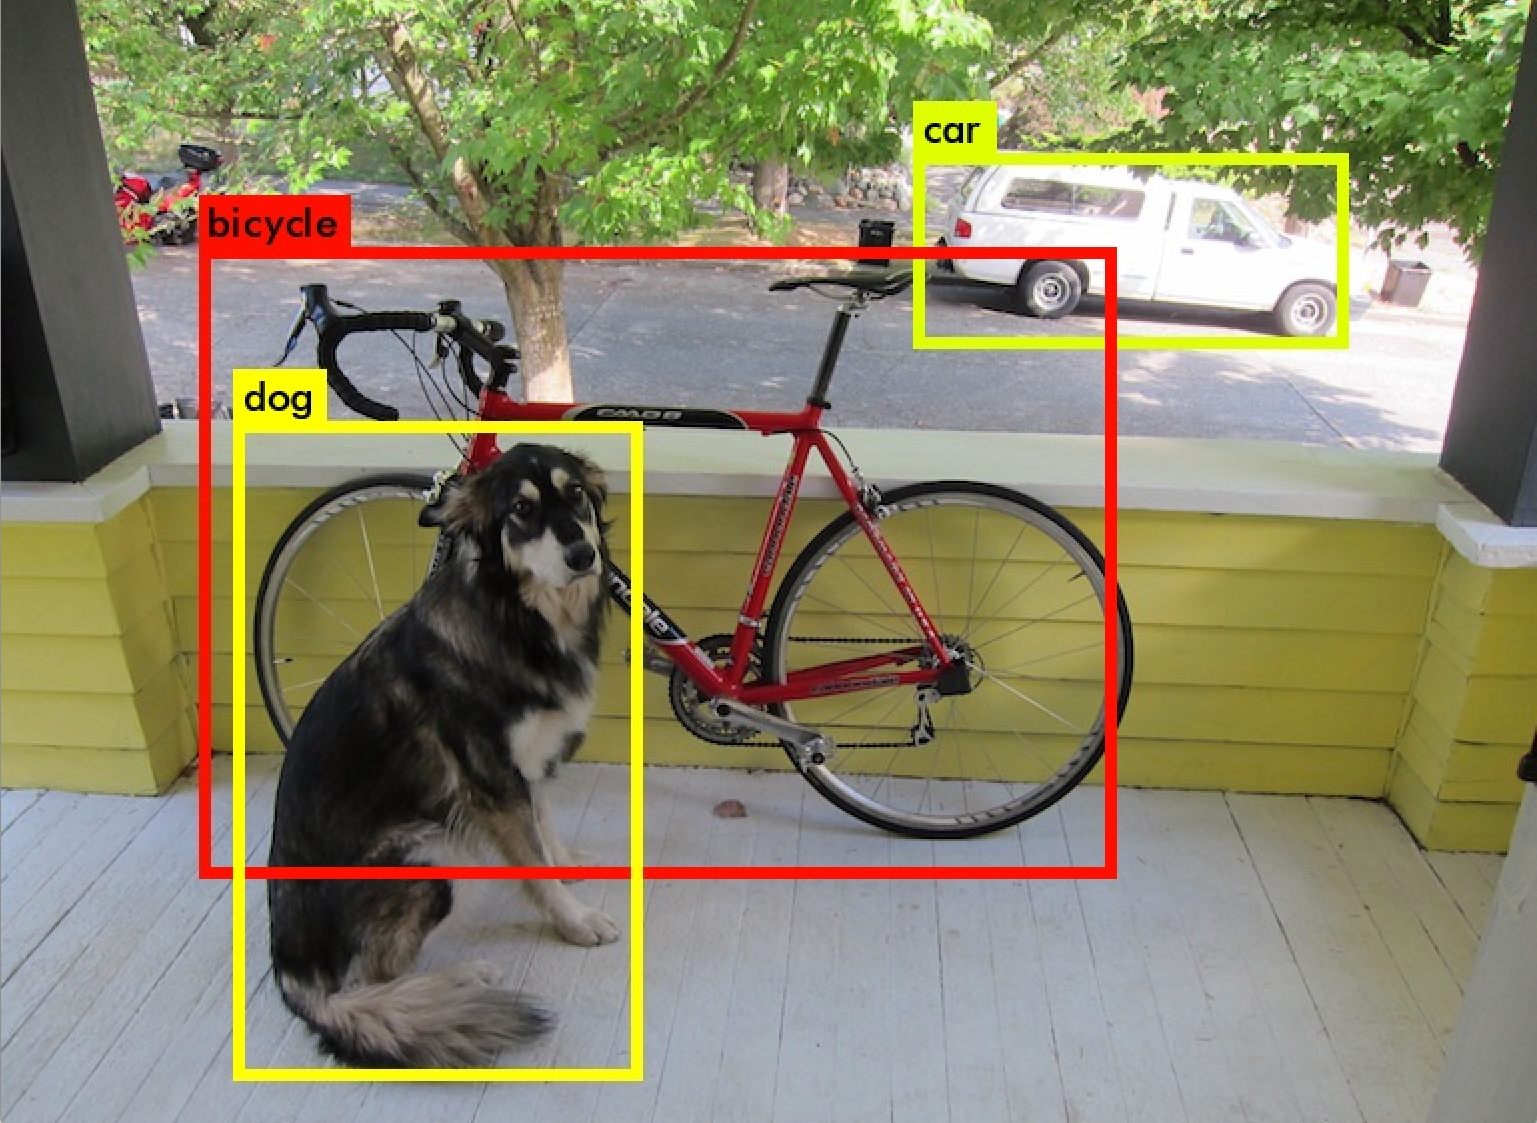
\includegraphics[width=0.3\textwidth]{images/computer_vision2.png}
    \end{subfigure}
\quad
    \centering
    \begin{subfigure}
        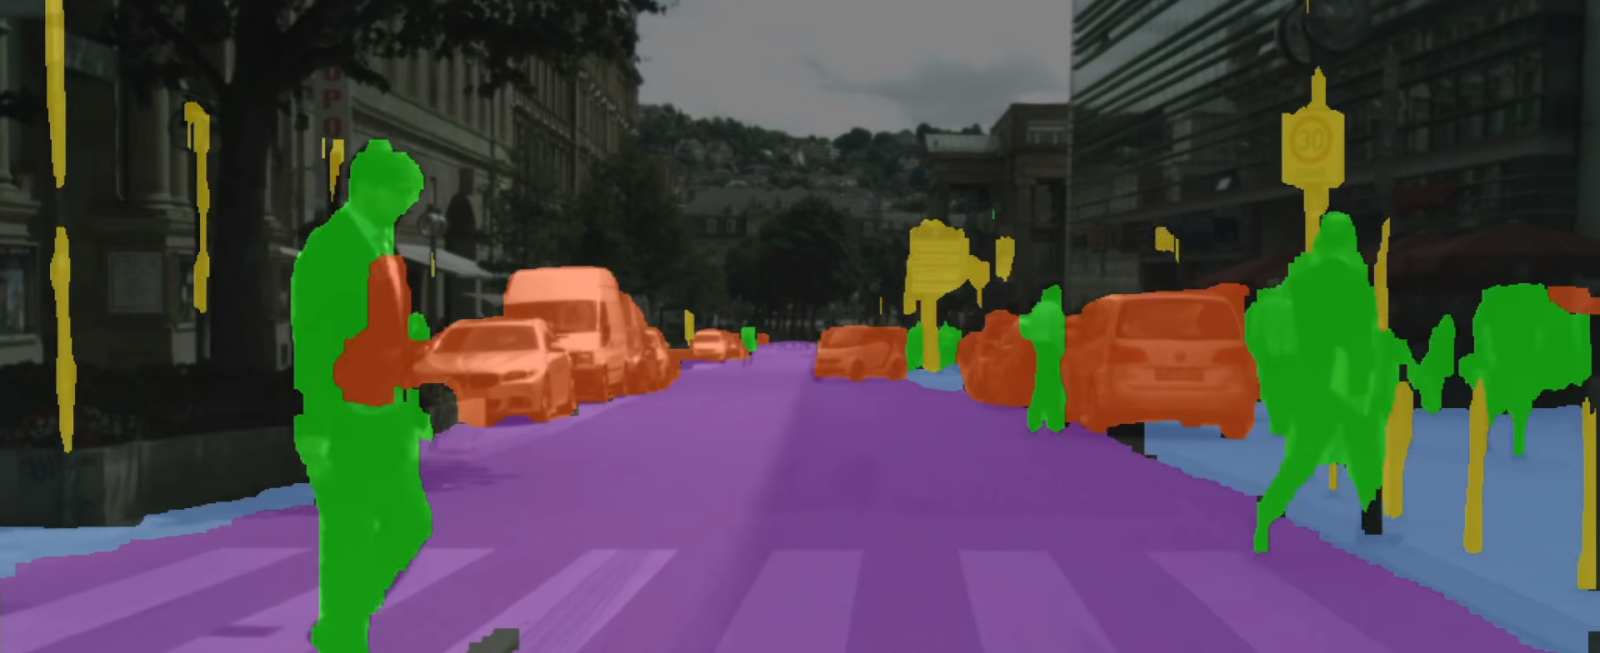
\includegraphics[width=0.5\textwidth]{images/computer_vision1.png}
    \end{subfigure}
\end{figure}
\end{frame}
%---------------------------------------------------------




%---------------------------------------------------------
\begin{frame}
\frametitle{Clasificación de imágenes}
\begin{figure}
    \centering
    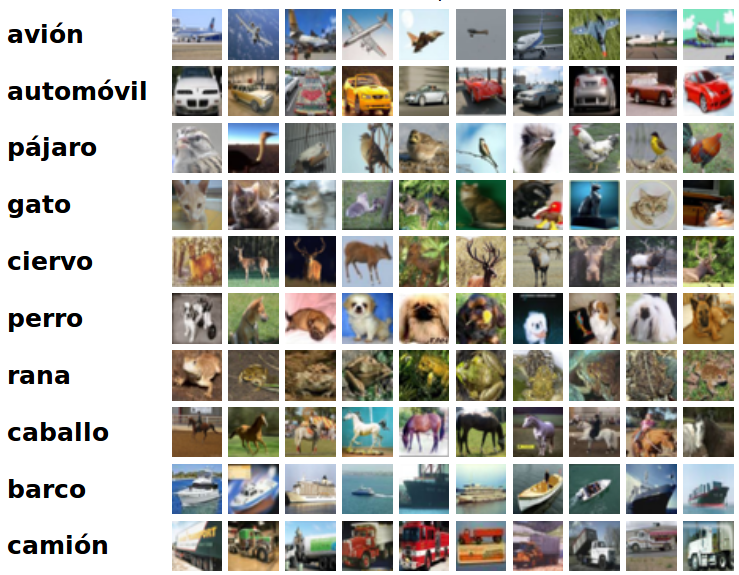
\includegraphics[width=0.6\textwidth]{images/ciphar10.png}
\end{figure}
\end{frame}
%---------------------------------------------------------




%---------------------------------------------------------
\begin{frame}[plain]
\frametitle{Representación de imágenes}
¿Qué es una imagen?
\begin{figure}
    \centering
    \includegraphics[width=0.7\textwidth]{images/image_representation.pdf}
\end{figure}
\end{frame}
%---------------------------------------------------------




%---------------------------------------------------------
\begin{frame}[plain]
\frametitle{Representación de imágenes}
Extracción de información de la imagen.
\vfill
Dependiente del dominio del problema.
\vfill
\begin{itemize}
    \item Textura
    \item Color
    \item Descriptores locales
\end{itemize}
\vfill
\begin{figure}
    \centering
    \includegraphics[width=0.9\textwidth]{images/descriptors.pdf}
\end{figure}
\vfill
Podemos obtener representaciones de imágenes, \(\boldsymbol{x} \in \boldsymbol{R^{D}}\)
\end{frame}
%---------------------------------------------------------





%---------------------------------------------------------
\begin{frame}
\frametitle{Clasificación de imágenes}

Conjunto de entrenamiento: \(\boldsymbol{x_i} \in \boldsymbol{R^{D}}\)
Anotaciones asociadas: \(\boldsymbol{y_i = 1\cdots K}\)\vfill

\vfill

\begin{equation}
    \boldsymbol{f(x_i, W)} = y_i \in \boldsymbol{1 \cdots K}
\end{equation}\pause

\vfill

\begin{itemize}
    \item SVM 
    \item Árboles de decisión 
    \item \textit{Bag of Words}
\end{itemize}

\end{frame}
%---------------------------------------------------------




%---------------------------------------------------------
\begin{frame}
\frametitle{Entrenamiento}
¿Cómo optimizar los parámetros \(W\)?
\vfill
\begin{equation}
    \boldsymbol{f(x_i, W)} = y_i \in \boldsymbol{1 \cdots K}
\end{equation}\pause
\vfill
Proceso iterativo:
\begin{itemize}
    \item Definir función de costo
    \item Minimizar la función de costo
\end{itemize}
\vfill
\end{frame}
%---------------------------------------------------------




%---------------------------------------------------------
\begin{frame}
\frametitle{Función de Costo}
Define un criterio de optimalidad que nos ayuda a
cuantificar cómo está actuando nuestro clasificador.
\vfill
\begin{equation}
\boldsymbol{L}(W) = \frac{1}{m} \sum^{m}_{i} L(f(x_i;W), y_i)
\end{equation}
\vfill
\end{frame}
%---------------------------------------------------------



%---------------------------------------------------------
\begin{frame}
\frametitle{Descenso de Gradiente Estocástico}
No tenemos control sobre nuestro conjunto de datos de entrenamiento, pero sí podemos modificar \(W\) para minimizar el costo.
\vfill
\begin{figure}
    \centering
    \includegraphics[width=0.6\textwidth]{images/gradient-descent.pdf}
\end{figure}
\vfill
\end{frame}
%---------------------------------------------------------





%---------------------------------------------------------
\begin{frame}
\frametitle{Descenso de Gradiente Estocástico}
Actualización de los pesos mediante el cómputo del costo en \textit{mini-batches}
\vfill
\begin{equation}
    W_{n+1} = W_n - \epsilon \frac{1}{m} \sum^{m}_{i} \nabla_{W_{n}} L(f(x_i; W_n), y_i)
\end{equation}
\vfill

\vfill
\end{frame}
%---------------------------------------------------------





%---------------------------------------------------------
\begin{frame}
\frametitle{Clasificación de imágenes}

Todos ampliamente superados por CNN

Pueden aprender representaciones \emph{Y} el modelo .
\begin{figure}
    \centering
    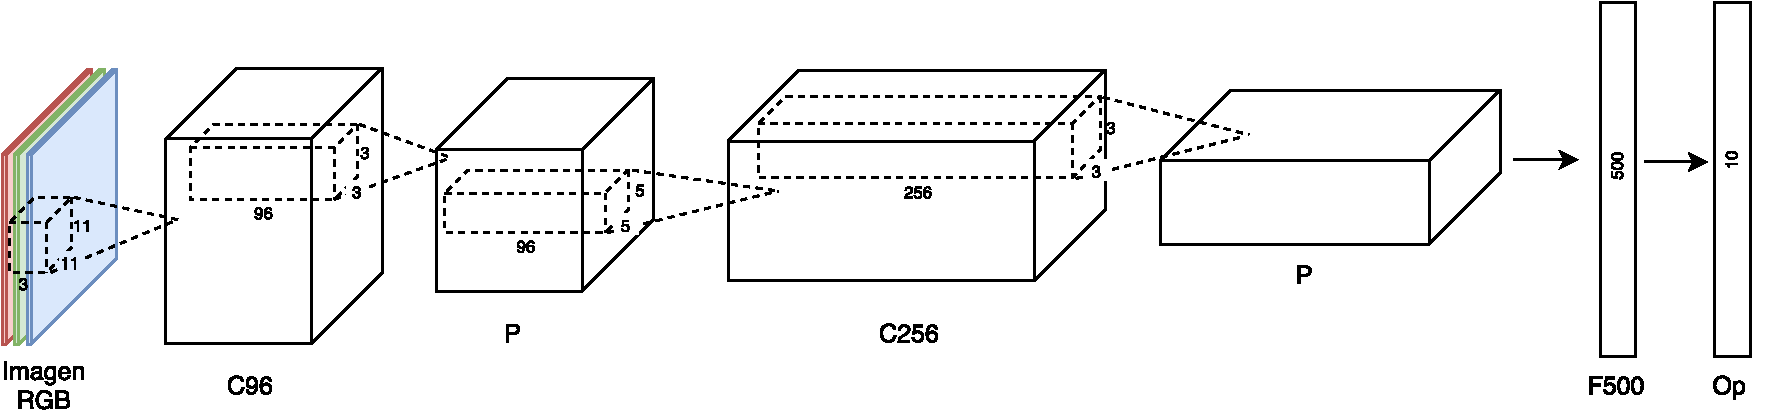
\includegraphics[width=\textwidth]{images/net_example.pdf}
\end{figure}
\end{frame}
%---------------------------------------------------------





%---------------------------------------------------------
\begin{frame}[plain]
\frametitle{Redes Neuronales}
\vfill
Unidades (neuronas) conectadas entre sí.
\vfill
Típicamente organizadas en capas.
\vfill
Neuronas de una capa interactúan con neuronas de la capa anterior.
\begin{figure}
    \centering
    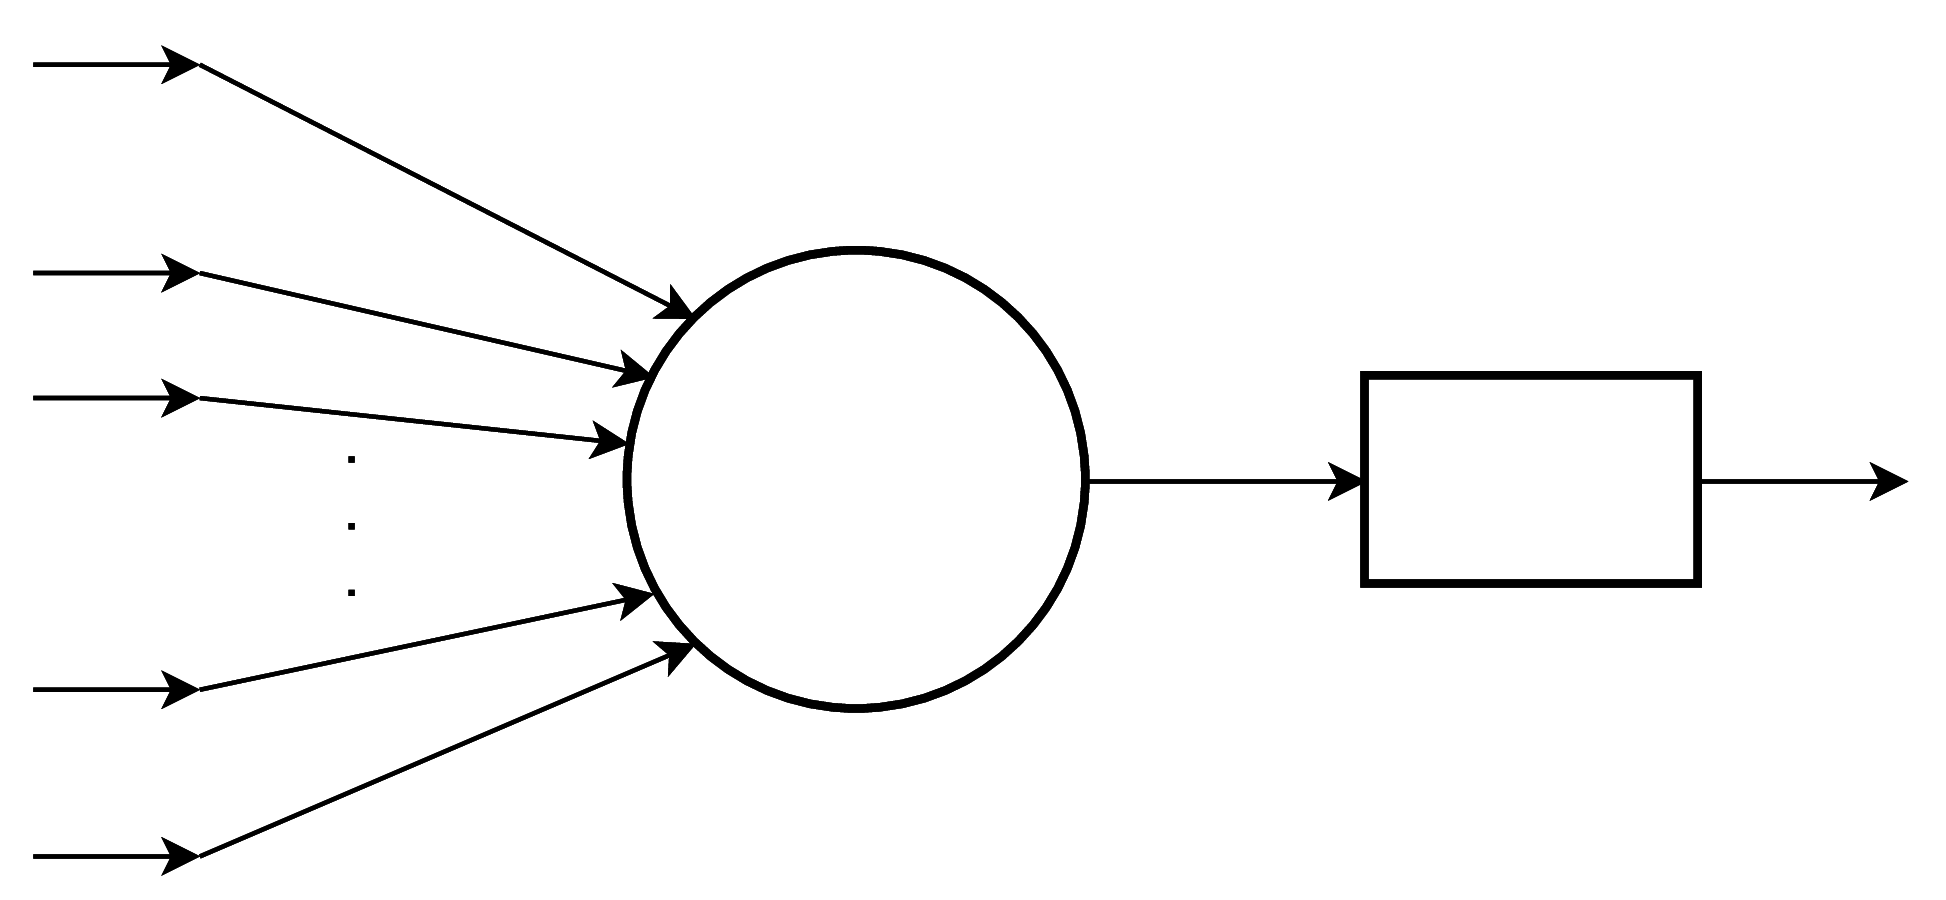
\includegraphics[width=\textwidth]{images/artificial-neuron.pdf}
\end{figure}
\end{frame}
%---------------------------------------------------------





%---------------------------------------------------------
\begin{frame}
\frametitle{Redes Neuronales}
\begin{figure}
    \centering
    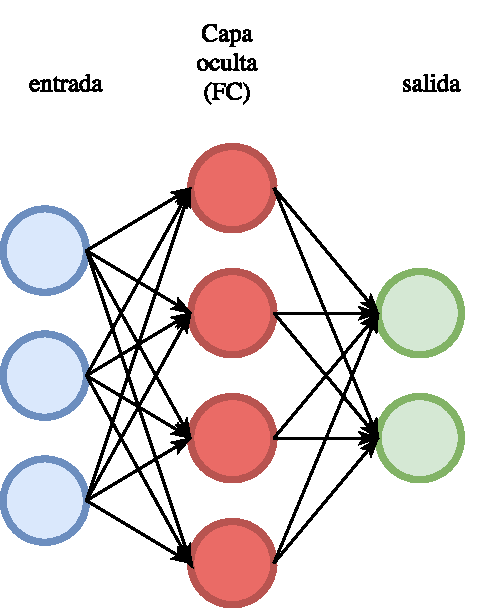
\includegraphics[width=0.4\textwidth]{images/neural-net.pdf}
\end{figure}
\end{frame}
%---------------------------------------------------------




%---------------------------------------------------------
\begin{frame}
\frametitle{Optimización: Retropropagación}
\vfill
Algoritmo utilizado para computar eficientemente el gradiente.
\vfill
\begin{enumerate}
    \item \textit{Forward pass}: cómputo del error
    \item \textit{Backward pass}: propagación del error a cada parámetro
\end{enumerate}
\vfill
Aplicación recursiva de la \textit{regla de la cadena}:
\vfill
\begin{equation}
    g(x,y,z) = \frac{x}{y^2} + z = \frac{x}{p} + z = q + z
\end{equation}
\vfill
\begin{figure}[H]
    \centering
    \tikzstyle{vertex}=[circle,fill=black!25,minimum size=20pt,inner sep=0pt]
    \tikzstyle{input}=[circle,draw=black,minimum size=20pt,inner sep=0pt]
    \tikzstyle{empty}=[circle,draw=white,minimum size=20pt,inner sep=0pt]
    \tikzstyle{emptyred}=[circle,draw=white,minimum size=20pt,inner sep=0pt,text=black!50!red]
    \tikzstyle{edgeup} = [draw,thick,->,above,sloped,color=black!50!green,text=black!50!green]
    \tikzstyle{arrow} = [->]
    \tikzstyle{edgedown} = [draw,thick,<-,below,sloped,color=black!50!red,text=black!50!red]
    \resizebox{0.9\textwidth}{!}{
        \begin{tikzpicture}[scale=1.5, auto,swap]
            % vertices
            \node[input] (x) at (-2,1) {$x$};
            \node[vertex] (div) at (2,1) {$/$};
            \node[vertex] (sum) at (4,1) {$+$};
            \node[empty] (output) at (5.7,1) {};
            \node[vertex] (pow) at (0,-1) {$\_^2$};
            \node[input] (y) at (-2,-1) {$y$};
            \node[input] (z) at (2,-1.5) {$z$};
            % edges forward
            \path[edgeup] (x.15) -- node[arrow] {$-3$} (div.165);
            \path[edgeup] (div.15) -- node[arrow] {$-0.75$} (sum.165);
            \path[edgeup] (pow.50) -- node[arrow] {$4$} (div.230);
            \path[edgeup] (z.50) -- node[arrow] {$4$} (sum.230);
            \path[edgeup] (y.15) -- node[arrow] {$2$} (pow.165);
            \path[edgeup] (sum) -- node[arrow] {$3.25$} (output);
            % edges backward
            \path[edgedown] (x.355) -- node[arrow] {$\frac{\partial q}{\partial x} = \frac{1}{y^2} = 0.25$} (div.185);
            \path[edgedown] (div.355) -- node[arrow] {$\frac{\partial g}{\partial q} = 1$} (sum.185);
            \path[edgedown] (pow.30) -- node[arrow] {$\frac{\partial q}{\partial p} = \frac{-x}{p^2} = -0.187$} (div.250);
            \path[edgedown] (z.30) -- node[arrow] {$\frac{\partial g}{\partial z} = 1$} (sum.250);
            \path[edgedown] (y.355) -- node[arrow] {$\frac{\partial p}{\partial y} = 2y = 4$} (pow.185);
            % final gradients
            \node[emptyred] (xback) at (-3.3,1) {$\frac{\partial g}{\partial x} = \frac{\partial g}{\partial q} \frac{\partial q}{\partial x} = 0.25$};
            \node[emptyred] (yback) at (-3.58,-1) {$\frac{\partial g}{\partial y} = \frac{\partial g}{\partial q} \frac{\partial q}{\partial p} \frac{\partial p}{\partial y} = -0.748$};
            \node[emptyred] (zback) at (1.35,-1.5) {$\frac{\partial g}{\partial z} = 1$};
        \end{tikzpicture}
    }
\end{figure}
\end{frame}
%---------------------------------------------------------





%---------------------------------------------------------
\begin{frame}
\frametitle{Redes Convolucionales}
Imagen como una función \(f:\mathbb{R}^2 \to \mathbb{R}^n\) 
\vfill

Un \textit{operador} toma una o más imágenes de entrada y produce una
imagen de salida.  
\vfill
	
Representamos a cada píxel como su posición en la imagen, \(\boldsymbol{x} = (i, j)\)
\vfill
	
Operador de píxeles:
\begin{equation}
g(i,j) = h(f(i,j))
\end{equation}
\vfill
\textit{filtro lineal} \textrightarrow \textit{operador local}
\end{frame}
%---------------------------------------------------------


%---------------------------------------------------------
\begin{frame}
\frametitle{Redes Convolucionales}
\begin{figure}
\centering
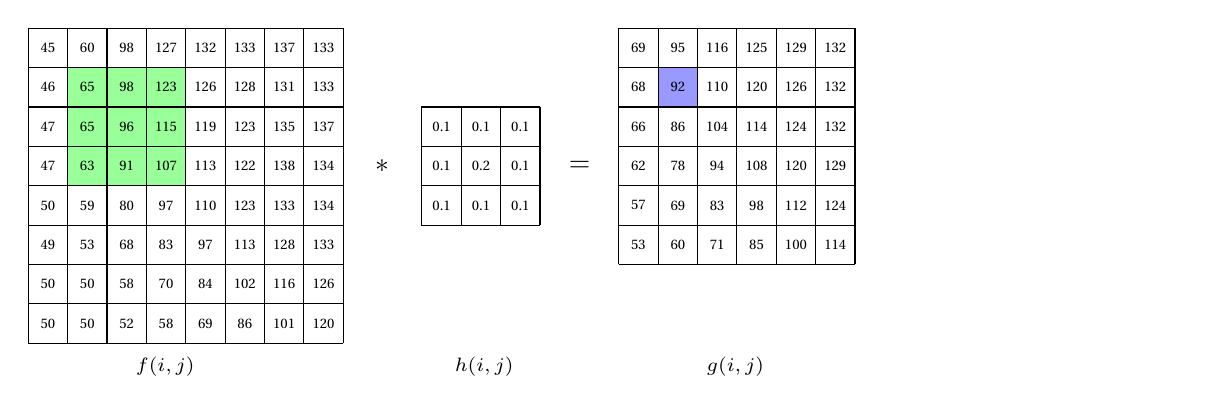
\begin{tikzpicture}[every node/.style={minimum size=.5cm-\pgflinewidth, outer sep=0pt}]
    \colorlet{gre}{green!40}
    \colorlet{blu}{blue!40}
    \node[fill=gre] at (-0.25,2.25)  {};
    \node[fill=gre] at (-0.25,1.75)  {};
    \node[fill=gre] at (-0.25,1.25)  {};
    \node[fill=gre] at (0.25,2.25)  {};
    \node[fill=gre] at (0.25,1.75)  {};
    \node[fill=gre] at (0.25,1.25)  {};
    \node[fill=gre] at (0.75,2.25)  {};
    \node[fill=gre] at (0.75,1.75)  {};
    \node[fill=gre] at (0.75,1.25)  {};
    % result fill
    \node[fill=blu] at (7.25, 2.25) {};
    \draw[step=0.5cm,color=black] (-1,-1) grid (3, 3);
    % first row
    \node at (-0.75,2.75) {\tiny 45};
    \node at (-0.25,2.75) {\tiny 60};
    \node at (0.25,2.75) {\tiny 98};
    \node at (0.75,2.75) {\tiny 127};
    \node at (1.25,2.75) {\tiny 132};
    \node at (1.75,2.75) {\tiny 133};
    \node at (2.25,2.75) {\tiny 137};
    \node at (2.75,2.75) {\tiny 133};
    % second row
    \node at (-0.75,2.25) {\tiny 46};
    \node at (-0.25,2.25) {\tiny 65};
    \node at (0.25,2.25) {\tiny 98};
    \node at (0.75,2.25) {\tiny 123};
    \node at (1.25,2.25) {\tiny 126};
    \node at (1.75,2.25) {\tiny 128};
    \node at (2.25,2.25) {\tiny 131};
    \node at (2.75,2.25) {\tiny 133};
    % third row
    \node at (-0.75,1.75) {\tiny 47};
    \node at (-0.25,1.75) {\tiny 65};
    \node at (0.25,1.75) {\tiny 96};
    \node at (0.75,1.75) {\tiny 115};
    \node at (1.25,1.75) {\tiny 119};
    \node at (1.75,1.75) {\tiny 123};
    \node at (2.25,1.75) {\tiny 135};
    \node at (2.75,1.75) {\tiny 137};
    % fourth row
    \node at (-0.75,1.25) {\tiny 47};
    \node at (-0.25,1.25) {\tiny 63};
    \node at (0.25,1.25) {\tiny 91};
    \node at (0.75,1.25) {\tiny 107};
    \node at (1.25,1.25) {\tiny 113};
    \node at (1.75,1.25) {\tiny 122};
    \node at (2.25,1.25) {\tiny 138};
    \node at (2.75,1.25) {\tiny 134};
    % fifth row
    \node at (-0.75,0.75) {\tiny 50};
    \node at (-0.25,0.75) {\tiny 59};
    \node at (0.25,0.75) {\tiny 80};
    \node at (0.75,0.75) {\tiny 97};
    \node at (1.25,0.75) {\tiny 110};
    \node at (1.75,0.75) {\tiny 123};
    \node at (2.25,0.75) {\tiny 133};
    \node at (2.75,0.75) {\tiny 134};
    % sixth row
    \node at (-0.75,0.25) {\tiny 49};
    \node at (-0.25,0.25) {\tiny 53};
    \node at (0.25,0.25) {\tiny 68};
    \node at (0.75,0.25) {\tiny 83};
    \node at (1.25,0.25) {\tiny 97};
    \node at (1.75,0.25) {\tiny 113};
    \node at (2.25,0.25) {\tiny 128};
    \node at (2.75,0.25) {\tiny 133};
    % seventh row
    \node at (-0.75,-0.25) {\tiny 50};
    \node at (-0.25,-0.25) {\tiny 50};
    \node at (0.25,-0.25) {\tiny 58};
    \node at (0.75,-0.25) {\tiny 70};
    \node at (1.25,-0.25) {\tiny 84};
    \node at (1.75,-0.25) {\tiny 102};
    \node at (2.25,-0.25) {\tiny 116};
    \node at (2.75,-0.25) {\tiny 126};
    % eight row
    \node at (-0.75,-0.75) {\tiny 50};
    \node at (-0.25,-0.75) {\tiny 50};
    \node at (0.25,-0.75) {\tiny 52};
    \node at (0.75,-0.75) {\tiny 58};
    \node at (1.25,-0.75) {\tiny 69};
    \node at (1.75,-0.75) {\tiny 86};
    \node at (2.25,-0.75) {\tiny 101};
    \node at (2.75,-0.75) {\tiny 120};
    % Convolution operator
    \node[text width=6cm, anchor=west, right] at (3.29,1.25) {$*$};
    % Filter (end right, end down)grid(start left, start up)
    \draw[step=0.5cm,color=black] (5.50,0.5) grid (3.994,2);
    % first row
    \node at (4.25, 1.75) {\tiny 0.1};
    \node at (4.75, 1.75) {\tiny 0.1};
    \node at (5.25, 1.75) {\tiny 0.1};
    % second row
    \node at (4.25, 1.25) {\tiny 0.1};
    \node at (4.75, 1.25) {\tiny 0.2};
    \node at (5.25, 1.25) {\tiny 0.1};
    % third row
    \node at (4.25, 0.75) {\tiny 0.1};
    \node at (4.75, 0.75) {\tiny 0.1};
    \node at (5.25, 0.75) {\tiny 0.1};
    % Equal
    \node[text width=6cm, anchor=west, right] at (5.75,1.25) {$=$};
    % Result
    \draw[step=0.5cm,color=black] (9.50,0) grid (6.4999,3);
    % first row
    \node at (6.75, 2.75) {\tiny 69};
    \node at (7.25, 2.75) {\tiny 95};
    \node at (7.75, 2.75) {\tiny 116};
    \node at (8.25, 2.75) {\tiny 125};
    \node at (8.75, 2.75) {\tiny 129};
    \node at (9.25, 2.75) {\tiny 132};
    % second row
    \node at (6.75, 2.25) {\tiny 68};
    \node at (7.25, 2.25) {\tiny 92};
    \node at (7.75, 2.25) {\tiny 110};
    \node at (8.25, 2.25) {\tiny 120};
    \node at (8.75, 2.25) {\tiny 126};
    \node at (9.25, 2.25) {\tiny 132};
    % third row
    \node at (6.75, 1.75) {\tiny 66};
    \node at (7.25, 1.75) {\tiny 86};
    \node at (7.75, 1.75) {\tiny 104};
    \node at (8.25, 1.75) {\tiny 114};
    \node at (8.75, 1.75) {\tiny 124};
    \node at (9.25, 1.75) {\tiny 132};
    % fourth row
    \node at (6.75, 1.25) {\tiny 62};
    \node at (7.25, 1.25) {\tiny 78};
    \node at (7.75, 1.25) {\tiny 94};
    \node at (8.25, 1.25) {\tiny 108};
    \node at (8.75, 1.25) {\tiny 120};
    \node at (9.25, 1.25) {\tiny 129};
    % fifth row
    \node at (6.75, 0.75) {\tiny 57};
    \node at (7.25, 0.75) {\tiny 69};
    \node at (7.75, 0.75) {\tiny 83};
    \node at (8.25, 0.75) {\tiny 98};
    \node at (8.75, 0.75) {\tiny 112};
    \node at (9.25, 0.75) {\tiny 124};
    % sixth row
    \node at (6.75, 0.25) {\tiny 53};
    \node at (7.25, 0.25) {\tiny 60};
    \node at (7.75, 0.25) {\tiny 71};
    \node at (8.25, 0.25) {\tiny 85};
    \node at (8.75, 0.25) {\tiny 100};
    \node at (9.25, 0.25) {\tiny 114};
    % Captions
    \node[text width=6cm, anchor=west, right] at (0.25,-1.30) {\scriptsize $f(i,j)$};
    \node[text width=6cm, anchor=west, right] at (4.30,-1.30) {\scriptsize $h(i,j)$};
    \node[text width=6cm, anchor=west, right] at (7.50,-1.30) {\scriptsize $g(i,j)$};
\end{tikzpicture}
\end{figure}
\end{frame}
%---------------------------------------------------------





%---------------------------------------------------------
\begin{frame}
\frametitle{Redes Convolucionales}
Convolución: localidad, reducción de parámetros, invarianza traslacional

Capas:
\begin{itemize}
    \item Convolucional
    \item Completamente conectada (FC)
    \item \textit{Pooling}. Usualmente \textit{MAX Pooling}
    \item \textit{Dropout}, ReLU, Softmax
\end{itemize}

\begin{figure}
\centering
\resizebox{.9\linewidth}{!}{
\begin{tabular}{cc}
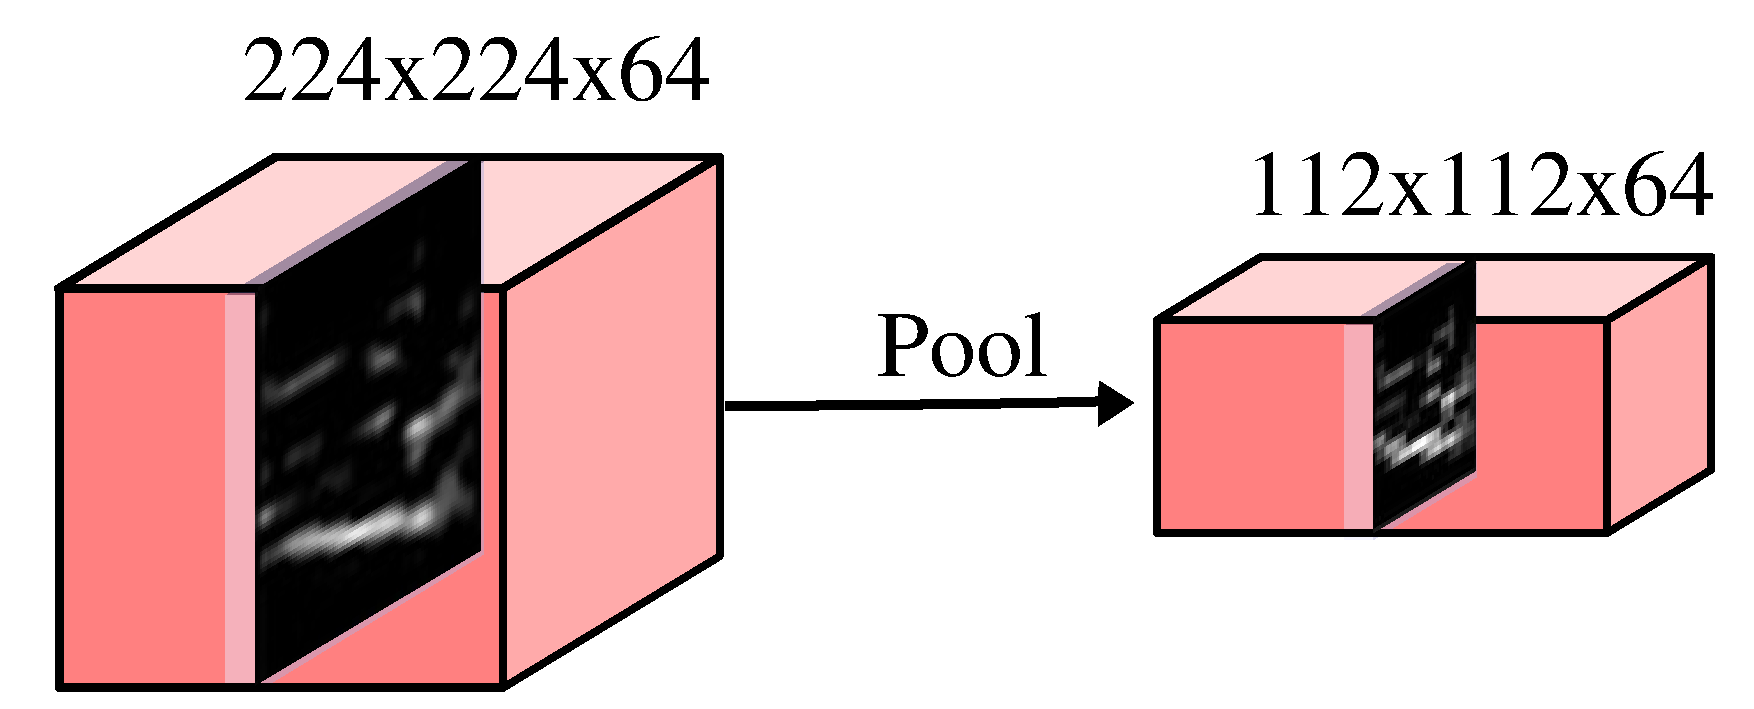
\includegraphics[width = 1.5in]{images/pool-layer.pdf} &
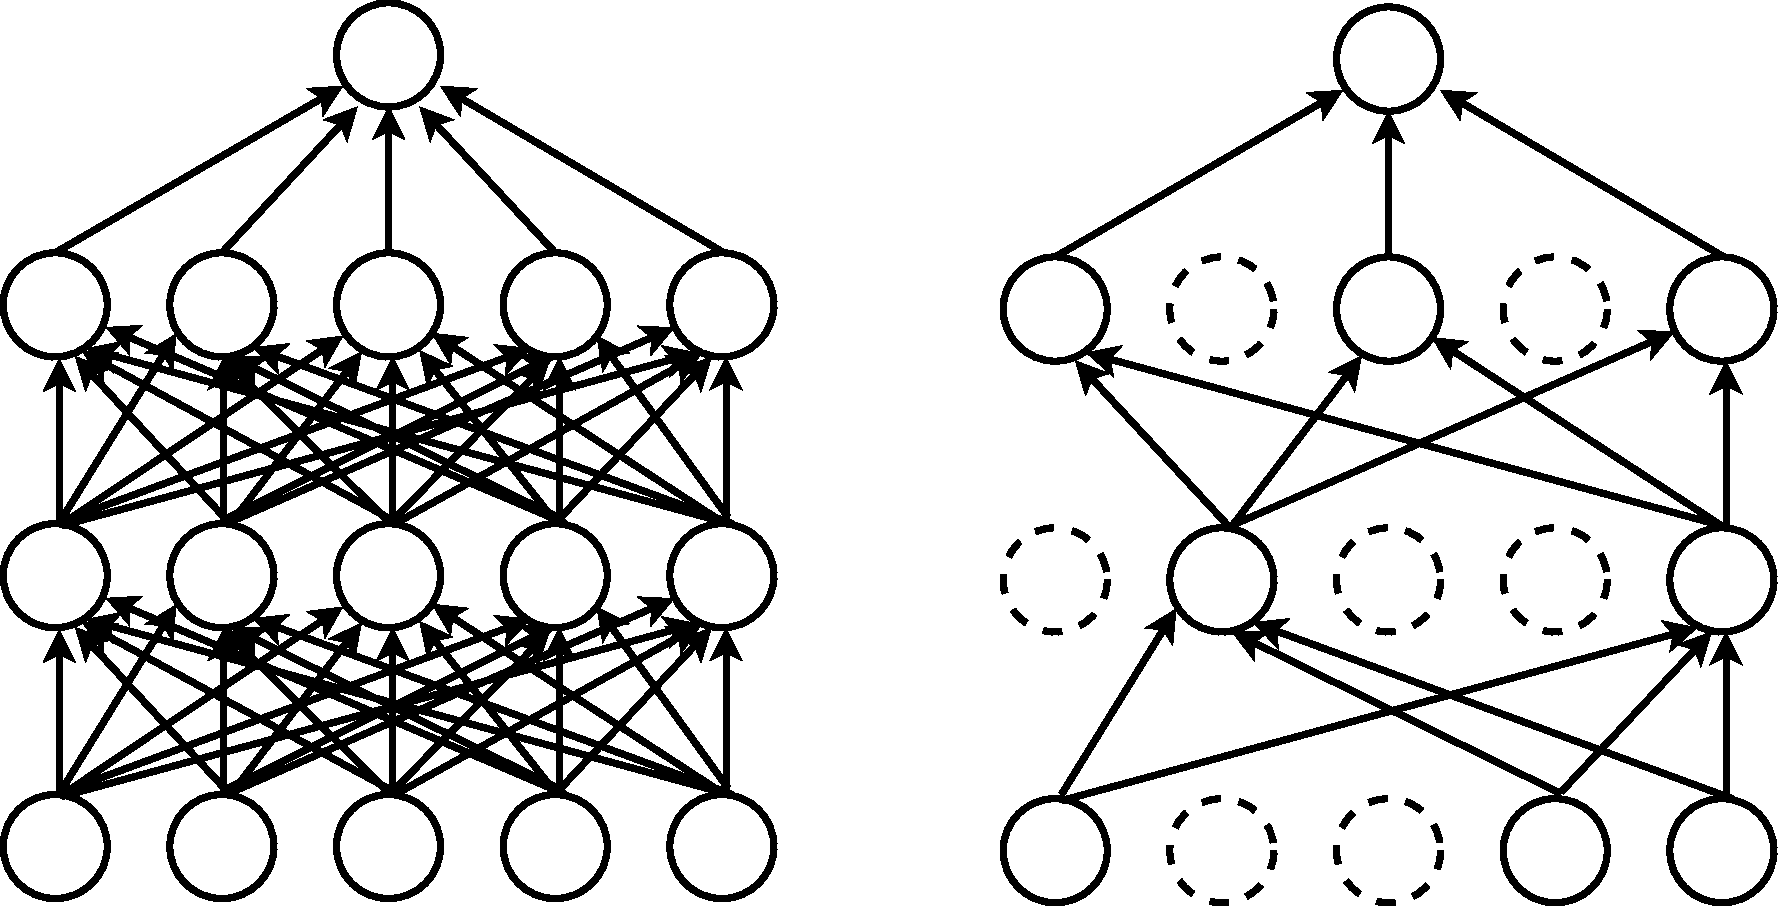
\includegraphics[width = 1.5in]{images/dropout.pdf} &
\end{tabular}
}
\end{figure}
\end{frame}
%---------------------------------------------------------





%---------------------------------------------------------
\begin{frame}
\frametitle{Redes Convolucionales}
Ejemplo: C96-P-C256-F500-Op.
\vfill
\begin{figure}
    \centering
    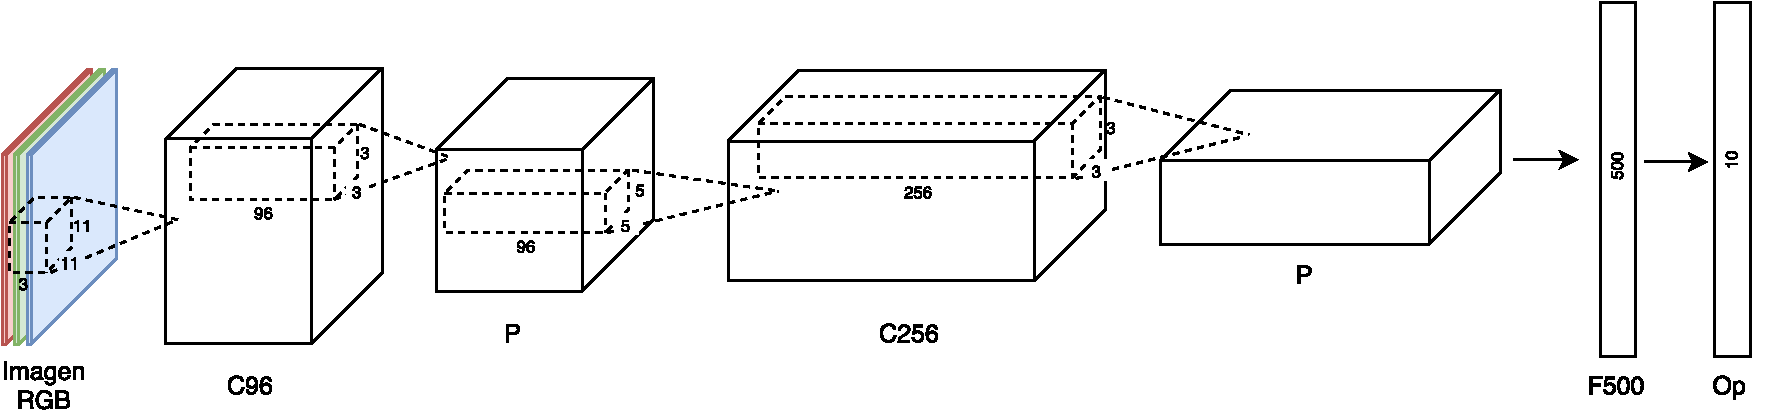
\includegraphics[width=\textwidth]{images/net_example.pdf}
\end{figure}
\vfill
Luego de cada capa convolucional se utilizan unidades ReLU y luego de cada capa completamente conectada se agrega una capa de \textit{Dropout} para prevenir sobreajuste de los datos.
\vfill
\end{frame}
%---------------------------------------------------------




%---------------------------------------------------------
\begin{frame}
\frametitle{(Algunos) problemas de Redes Convolucionales}
\begin{itemize}
    \item Requieren grandes conjuntos de datos
    \item Conjuntos de datos específicos a un dominio
    \item Anotaciones manuales son muy costosas
\end{itemize}
\end{frame}
%---------------------------------------------------------




\section{pretext}
%---------------------------------------------------------
\begin{frame}
\frametitle{Entrenamiento mediante tareas de pretexto}
Tareas de pretexto \\\vfill

No son útiles en si mismas, pero sirven para aprender representaciones generales que puedan ser aplicadas a otro problema.\\\vfill
	
\begin{itemize}
    \item reconstrucción de la imagen de entrada
    \item predicción de píxeles en una secuencia de video 
    \item ordenamiento temporal de cuadros de videos
    \item ordenamiento parches en imágenes estáticas
\end{itemize}\\
\vfill

Anotaciones fáciles de obtener e incluso a partir del mismo conjunto de datos. \\
\vfill
La hipótesis es que el modelo aprenderá características de alto nivel para poder realizar su tarea.
\vfill
\end{frame}
%---------------------------------------------------------






%---------------------------------------------------------
\begin{frame}
\frametitle{Automovimiento}
\vfill
un agente móvil puede valerse de la información obtenida de su propio movimiento para
supervisar el aprendizaje de buenas representaciones visuales de su
entorno.
\vfill
¿Podemos predecir cuando dos fotos son la misma a pesar haber sufrido alguna transformación?\\

\vfill

\begin{itemize}
    \item tarea de clasificación donde el objetivo es predecir la transformación 
\end{itemize}

\vfill

\begin{block}{Información Odométrica}
Información sobre el cambio de posición respecto a un punto inicial.
\end{block}
\vfill
\end{frame}
%---------------------------------------------------------





%---------------------------------------------------------
\begin{frame}
\frametitle{Automovimiento}

¿Como sabemos si cuando son buenas representaciones?\\\pause

\vfill
\begin{enumerate}
    \item la capacidad de poder realizar múltiples tareas visuales
    \item la habilidad de poder aprender nuevas tareas visuales basándose en pocos ejemplos.
\end{enumerate}\pause
\vfill

\begin{block}{}
El problema de relacionar los estímulos visuales con el automovimiento puede ser establecido como el problema de predecir las transformaciones de la cámara en pares de imágenes a lo largo del movimiento de la misma
\end{block}
\vfill
\end{frame}
%---------------------------------------------------------




%---------------------------------------------------------
\begin{frame}[plain]
\frametitle{Automovimiento}
El problema puede ser planteado con redes siamesas\\
\vfill
\begin{figure}
    \centering
    \includegraphics[width=\textwidth]{images/siamese-example_kitti.pdf}
\end{figure}
\vfill
\end{frame}
%---------------------------------------------------------







%---------------------------------------------------------
\begin{frame}
\frametitle{\textit{Slow Feature Analysis}}

Técnica de aprendizaje no supervisado:
\begin{itemize}
    \item \textit{features} cambian poco en una ventana de tiempo pequeña \pause
	\end{itemize}

	Sean \(x_{t_1}\) y \(x_{t_2}\) representaciones de imágenes en tiempos \(t_1\) y \(t_2\)\\
Sea \(D\) una medida de similitud. Podemos definir una función de costo:

\begin{equation}
L(x_{t_1}, x_{t_2}, W) = \begin{cases}
                           D(x_{t_1}, x_{t_2}),& \text{si} |t_1 - t_2| \leq T \\ 
                           \max{(0, m - D(x_{t_1}, x_{t_2}))},& \text{si} |t_1 - t_2| > T
                         \end{cases}
\end{equation}

\(W\) son los parámetros compartidos de las redes siamesas\\
\(m\) es el margen mínimo que debe separar a las representaciones distintas.
\end{frame}
%---------------------------------------------------------





%---------------------------------------------------------
\begin{frame}
\frametitle{Automovimiento}
\begin{figure}
    \centering
    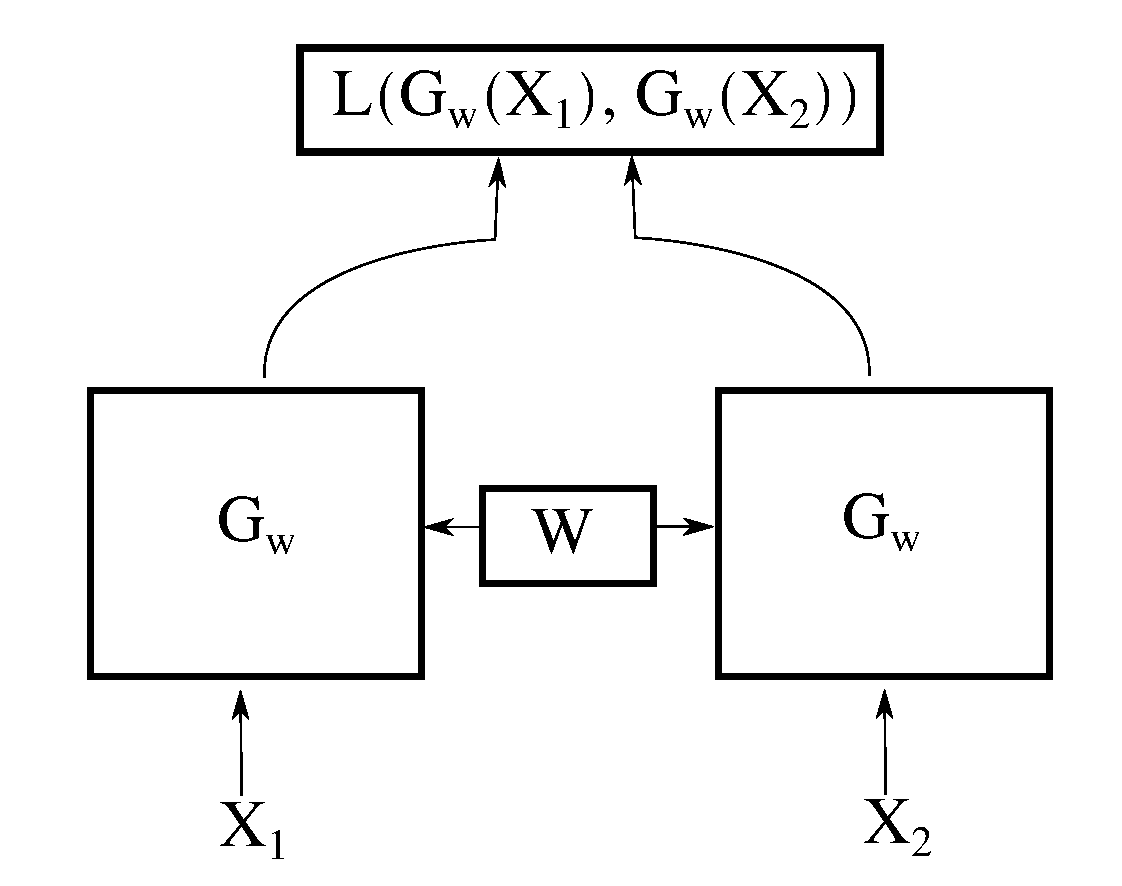
\includegraphics[width=0.5\textwidth]{images/siamese-diagram.pdf}
\end{figure}
\end{frame}
%---------------------------------------------------------





%---------------------------------------------------------
\begin{frame}
\frametitle{\textit{Slow Feature Analysis}}
\begin{figure}
    \centering
    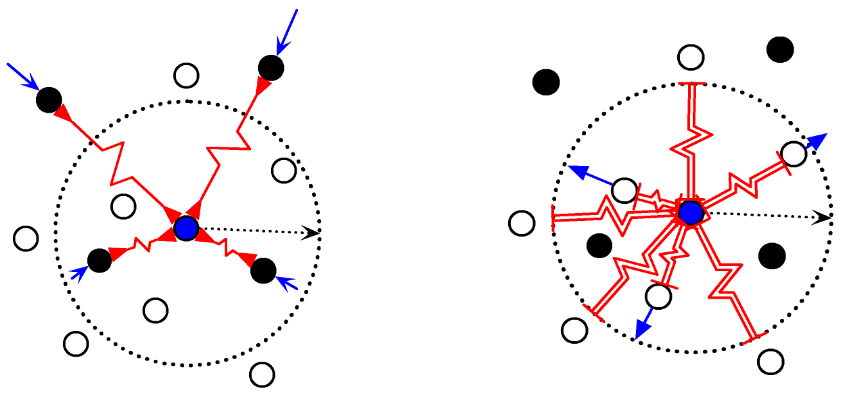
\includegraphics[width=0.8\textwidth]{images/example_contrastiveloss.png}
\end{figure}
\end{frame}
%---------------------------------------------------------





%---------------------------------------------------------
\begin{frame}
\frametitle{Información odométrica para entrenar redes siamesas}
\begin{itemize}
    \item Tarea de clasificación: predecir transformaciones en \(X, Y, Z\)
    \item Transformaciones en espacio continuo 
    \item 3 clasificadores con categorías discretizadas
\end{itemize}
\end{frame}
%---------------------------------------------------------





\section{Experimentos}
%---------------------------------------------------------
\begin{frame}
\frametitle{Experimentos - Diseño}
\begin{enumerate}
    \item Particionado del conjunto de entrenamiento
    \item Hiperparámetros
    \item Preentrenamiento inicial
    \item Transferencia de aprendizaje
    \item Chequeo de métricas
\end{enumerate}
\end{frame}
%---------------------------------------------------------





%---------------------------------------------------------
\begin{frame}
\frametitle{Experimentos - Prueba de concepto: MNIST}
Conjunto de datos de dígitos manuscritos
\vfill
Pares artificiales con traslaciones en X e Y, rotaciones en Z
\vfill
\begin{figure}
\centering
\resizebox{.9\linewidth}{!}{
\begin{tabular}{cccccc}

\includegraphics[width = 1.5in]{./images/mnist/a1.png} &

\includegraphics[width = 1.5in]{./images/mnist/a.png} &

\includegraphics[width = 1.5in]{./images/mnist/b1.png} &

\includegraphics[width = 1.5in]{./images/mnist/b.png} &

\includegraphics[width = 1.5in]{./images/mnist/c.png} &

\includegraphics[width = 1.5in]{./images/mnist/c1.png}\\
\end{tabular}
}
\label{fig:mnist-sample}
\end{figure}
\vfill
\begin{itemize}
	\item Traslaciones de [-3, 3] píxeles en X, Y
	\item Rotaciones de [-30, 30] grados en Z
	\item Para SFA, se consideran cercanos las imágenes en [-1,1], [-3, 3] grados  
\end{itemize}

\end{frame}
%---------------------------------------------------------





%---------------------------------------------------------
\begin{frame}[plain]
\frametitle{Experimentos - Prueba de concepto: MNIST}
\begin{figure}
    \centering
    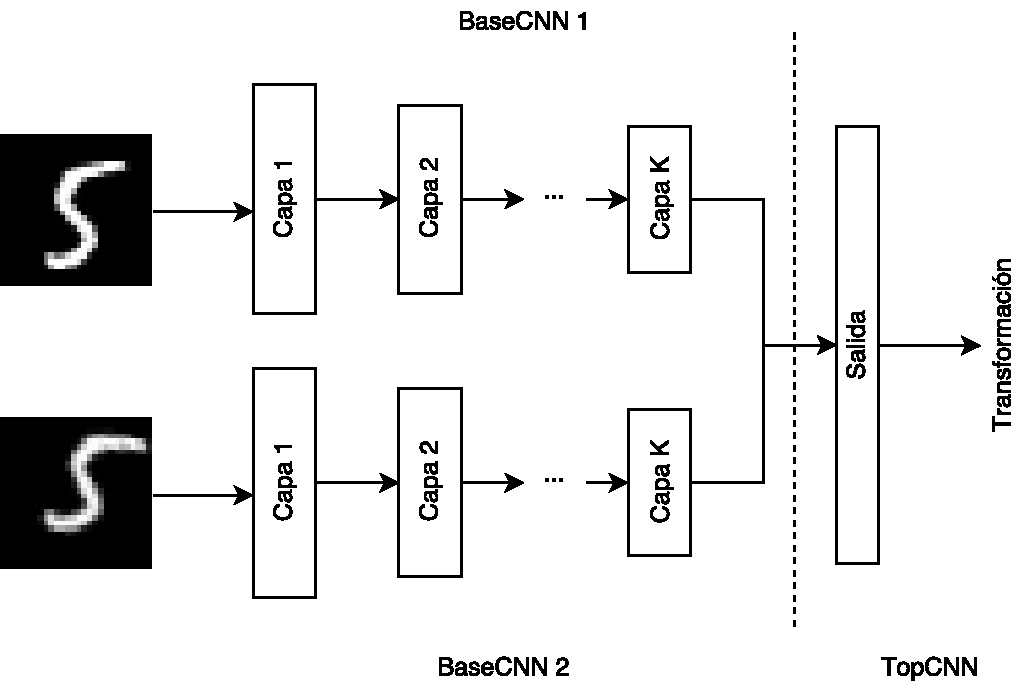
\includegraphics[width=0.9\textwidth]{images/siamese-example.pdf}
\end{figure}
\end{frame}
%---------------------------------------------------------






%---------------------------------------------------------
\begin{frame}
\frametitle{Experimentos - Prueba de concepto: MNIST}
\begin{itemize}
    \item Componentes siameses: C96-P-C256-P, Concatenación de representaciones: F1000-D-Op.
    \item 40K iteraciones, márgenes 10 y 100 para SFA
    \item 5 millones de pares de imágenes
    \item Partición en entrenamiento-validación
    \item Transferencia de aprendizaje: se congelaron las capas convolucionales.
\end{itemize}
\vfill
\begin{block}{Métricas}
Accuracy, Función de costo durante entrenamiento
\end{block}
\end{frame}
%---------------------------------------------------------





%---------------------------------------------------------
\begin{frame}
\frametitle{Experimentos - Prueba de concepto: MNIST}
\begin{table}
\centering
\begin{tabular}{l|rrrr}
\hline
\multicolumn{1}{r}{}
& \multicolumn{4}{c}{datos entrenamiento}
& \multicolumn{1}{l}{Método}
& \multicolumn{1}{r}{100}
& \multicolumn{1}{r}{300}
& \multicolumn{1}{r}{1000}
& \multicolumn{1}{r}{10000} \\ \cline{1-5}
\hline
Desde cero & 0.42 & 0.70 & 0.82 & 0.97\\
SFA(m=10) & 0.52 & 0.71 & 0.77 & 0.82\\
SFA(m=100) & 0.58 & 0.73 & 0.80 & 0.88\\
Automovimiento & 0.75 & 0.90 & 0.92 & 0.99\\
\hline
\end{tabular}
\end{table}
\end{frame}
%---------------------------------------------------------





%---------------------------------------------------------
\begin{frame}
\frametitle{Experimentos - KITTI}
\vfill
11 secuencias que registran el movimiento de un automóvil en una ciudad\vfill
\begin{figure}
\centering
\resizebox{.9\linewidth}{!}{
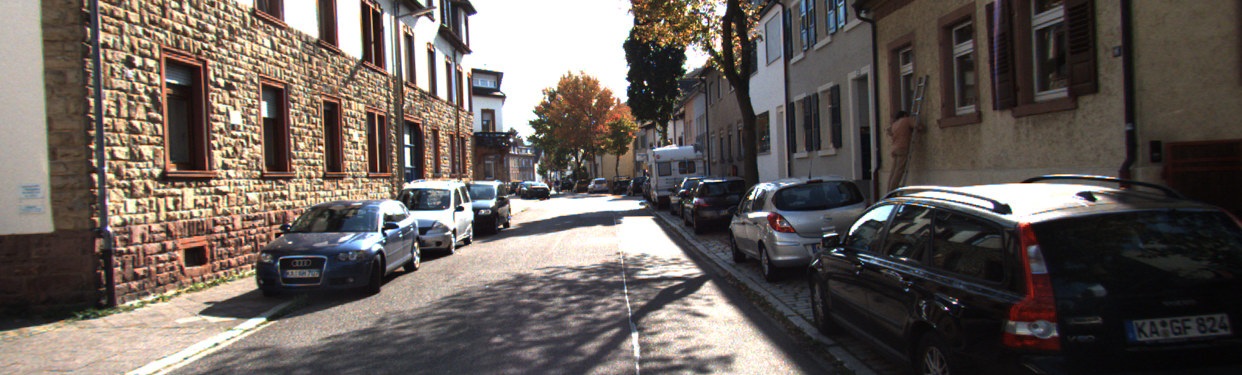
\includegraphics[width = 1.5in]{./images/kitti/original.png} &
}
\end{figure}
\vfill
\begin{itemize}
    \item Matrices de rotación Las transformaciones en X, Y y Z en base a las matrices de rotación provistas por los creadores del conjunto de datos.
    \item Para las rotaciones en el eje Y se calculó el ángulo correspondiente al cambio entre dos \textit{frames}.
    \item Discretización de traslaciones y rotaciones en categorías
\end{itemize}
\vfill
\end{frame}
%---------------------------------------------------------





%---------------------------------------------------------
\begin{frame}
\frametitle{KITTI - Pares de entrenamiento}
\begin{figure}
\centering
\resizebox{.9\linewidth}{!}{
\begin{tabular}{cccccc}
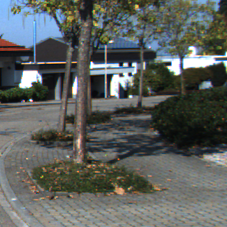
\includegraphics[width = 1.5in]{./images/kitti/a.png} &

\includegraphics[width = 1.5in]{./images/kitti/a1.png} &
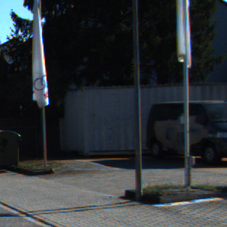
\includegraphics[width = 1.5in]{./images/kitti/b.png} &

\includegraphics[width = 1.5in]{./images/kitti/b1.png} &
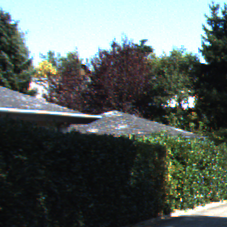
\includegraphics[width = 1.5in]{./images/kitti/c.png} &
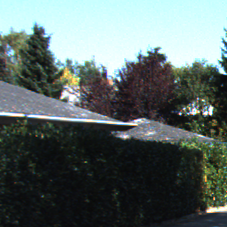
\includegraphics[width = 1.5in]{./images/kitti/c1.png}\\
\end{tabular}
}
\label{fig:kitti-sample}
\end{figure}
\vfill
\begin{itemize}
    \item Clasificación, 20 clases por eje
    \item Automovimiento: cuadros separados a lo sumo por 7 cuadros intermedios.
    \item SFA: ±7 cuadros considerados cercanos
    \item Se extrayeron parches aleatorios de \(227 \times 227\)
\end{itemize}
\vfill
\end{frame}
%---------------------------------------------------------





%---------------------------------------------------------
\begin{frame}[plain]
\frametitle{KITTI - Entrenamiento}
\vfill
\begin{itemize}
    \item Red: AlexNet
    \item Pre-entrenamiento 60K iteraciones
    \item Transferencia de aprendizaje: 10K iteraciones
\end{itemize}\pause
\vfill
\begin{block}{Baseline}
Se entrenó AlexNet con el conjunto de datos ILSVRC'12 desde cero utilizando 20 y 1000 imágenes por clase (ALEX-20 y ALEX-1000)\\
Las redes siamesas fueron entrenadas con aproximadamente 20K pares de imágenes.
\end{block}\pause
\vfill
\end{frame}
%---------------------------------------------------------





%---------------------------------------------------------
\begin{frame}
\frametitle{Experimentos - KITTI + SUN397}
397 categorías de paisajes interiores y exteriores\vfill
3 particiones con datos de entrenamiento-validación\vfill
\begin{figure}
\centering
\resizebox{.7\linewidth}{!}{
\begin{tabular}{cccc}
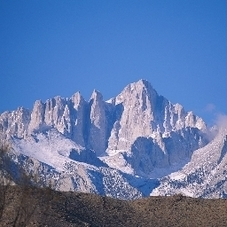
\includegraphics[width = 1.5in]{./images/sun397/mountain_snowy.jpg} &
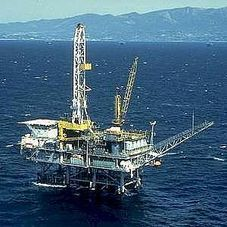
\includegraphics[width = 1.5in]{./images/sun397/oilrig.jpg} &
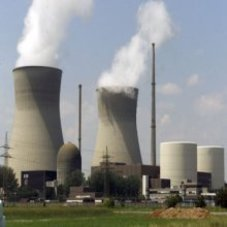
\includegraphics[width = 1.5in]{./images/sun397/nuclear_power_plant.jpg} &
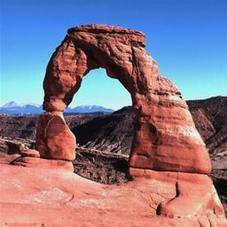
\includegraphics[width = 1.5in]{./images/sun397/rock_arch.jpg} \\
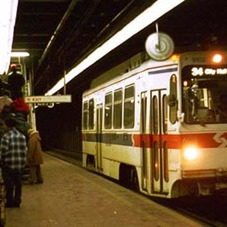
\includegraphics[width = 1.5in]{./images/sun397/subway_station.jpg} &
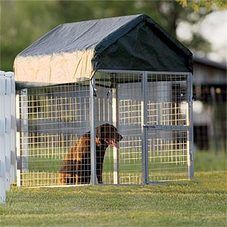
\includegraphics[width = 1.5in]{./images/sun397/kennel.jpg} &
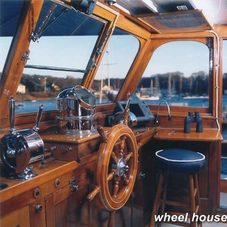
\includegraphics[width = 1.5in]{./images/sun397/pilothouse.jpg} &
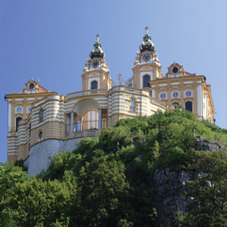
\includegraphics[width = 1.5in]{./images/sun397/abbey.jpg} \\
\end{tabular}
}
\end{figure}
\end{frame}
%---------------------------------------------------------





%---------------------------------------------------------
\begin{frame}
\frametitle{Experimentos - KITTI + SUN397}
Preentrenamiento: automovimiento, SFA y pesos aleatorios.
\vfill
Transferencia de aprendizaje con SUN397 con 5 y 20 elementos por categoría.
\vfill
Calidad de las representaciones: \textit{Softmax} para cada capa\pause
\vfill
Accuracy:
\begin{table}
\centering
\resizebox{\textwidth}{!}{
\begin{tabular}{l|r|r|ccccc|r|ccccc}
\hline
\multicolumn{1}{l}{Método}
& \multicolumn{1}{r}{\#preentr.}
& \multicolumn{1}{r}{\#finet.}
& \multicolumn{1}{c}{L1}
& \multicolumn{1}{c}{L2}
& \multicolumn{1}{c}{L3}
& \multicolumn{1}{c}{L4}
& \multicolumn{1}{c}{L5}
& \multicolumn{1}{r}{\#finet.}
& \multicolumn{1}{c}{L1}
& \multicolumn{1}{c}{L2}
& \multicolumn{1}{c}{L3}
& \multicolumn{1}{c}{L4}
& \multicolumn{1}{c}{L5} \\ \cline{1-14}
\hline

ALEX-1000 & 1M & 5 & 3.73 & 5.07 & 5.07 & 8.53 & 10.40 & 20 & 9.07 & 12.53 & 16.27 & 17.60 & 10.67\\
ALEX-20 & 20K & 5 & 2.93 & 1.87 & 3.73 & 5.07 & 3.20 & 20 & 6.13 & 5.33 & 5.33 & 4.53 & 5.07\\
KITTI-SFA & 20.7K & 5 & 2.13 & 3.20 & 2.40 & 1.60 & 1.87 & 20 & 4.53 & 3.73 & 2.13 & 2.40 & 2.93\\
KITTI-AUT & 20.7K & 5 & 2.93 & 1.87 & 3.20 & 5.87 & 1.33 & 20 & 6.67 & 7.47 & 9.87 & 9.33 & 4.00\\

\hline
\end{tabular}
}
\end{table}
\vfill
\end{frame}
%---------------------------------------------------------





%---------------------------------------------------------
\begin{frame}
\frametitle{Experimentos - KITTI + ImageNet}
Conjunto de datos ILSVRC'12, 1000 categorías
\begin{figure}
\centering
\resizebox{.75\linewidth}{!}{
\begin{tabular}{cccc}
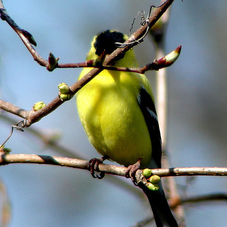
\includegraphics[width = 1.5in]{./images/imagenet/n01531178_108.JPEG} &
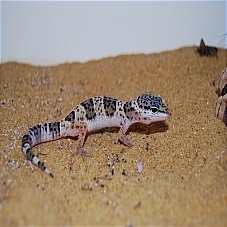
\includegraphics[width = 1.5in]{./images/imagenet/n01675722_126.JPEG} &
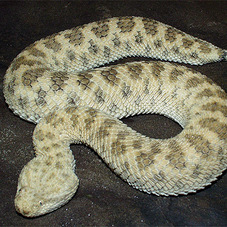
\includegraphics[width = 1.5in]{./images/imagenet/n01753488_177.JPEG} &
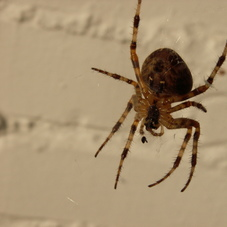
\includegraphics[width = 1.5in]{./images/imagenet/n01773797_48.JPEG} \\
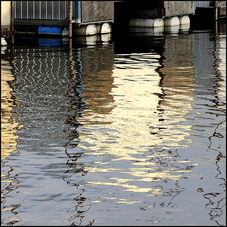
\includegraphics[width = 1.5in]{./images/imagenet/n02859443_1229.JPEG} &
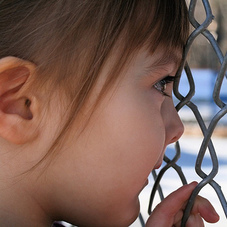
\includegraphics[width = 1.5in]{./images/imagenet/n03000134_789.JPEG} &
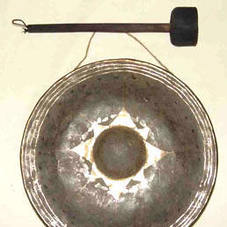
\includegraphics[width = 1.5in]{./images/imagenet/n03017168_743.JPEG} &
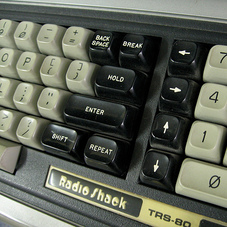
\includegraphics[width = 1.5in]{./images/imagenet/n03085013_2149.JPEG} \\
\end{tabular}
}
\end{figure}
\vfill
Se crearon conjuntos de datos con 1 5, 10, 20 y 1000 imágenes por categoría
\vfill
\end{frame}
%---------------------------------------------------------





%---------------------------------------------------------
\begin{frame}
\frametitle{Experimentos - KITTI + ImageNet}

Preentrenamiento con automovimiento, SFA y pesos aleatorios.\pause
\vfill
Transferencia de aprendizaje con ImageNet.\pause
\vfill

Accuracy:
\begin{table}
\centering
\begin{tabular}{l|ccccc}
\hline
\multicolumn{1}{l}{Método}
& \multicolumn{1}{c}{1}
& \multicolumn{1}{c}{5}
& \multicolumn{1}{c}{10}
& \multicolumn{1}{c}{20}
& \multicolumn{1}{c}{1000} \\ \cline{1-6}
\hline

KITTI-AUT & 0.49 & 1.27 & 2.14 & 4.13 & 20.8\\
KITTI-SFA & 0.35 & 0.75 & 1.34 & 2.64 & 11.83\\
ALEXNET & 0.45 & 0.95 & 1.91 & 3.69 & 18.35\\

\hline
\end{tabular}
\end{table}
\end{frame}
%---------------------------------------------------------





%---------------------------------------------------------
\begin{frame}
\frametitle{Conclusiones}
\begin{itemize}
    \item \textit{automovimiento} permite obtener  resultados equiparables al estado del arte.
    \item Anotaciones de automovimiento fáciles de obtener. 
    \item Bajo la misma cantidad de imágenes de entrenamiento, \textit{automovimiento} equipara a técnicas supervisadas de clasificación.
\end{itemize}
\end{frame}
%---------------------------------------------------------





%---------------------------------------------------------
\begin{frame}
\frametitle{Trabajo a Futuro}
\begin{itemize}
    \item Probar otras variantes: arquitecturas de redes, conjuntos de datos
    \item ¿Puede el \textit{automovimiento} aplicarse a otros dominios?
    \item Evaluar la utilidad de otras tareas de pretexto
\end{itemize}
\end{frame}
%---------------------------------------------------------





%---------------------------------------------------------
\begin{frame}
\frametitle{}
\vfill
\centering
	¿Preguntas?
\vfill
\end{frame}
%---------------------------------------------------------





%---------------------------------------------------------
\begin{frame}
\frametitle{}
\vfill
\centering
    Gracias!
\vfill
\end{frame}
%---------------------------------------------------------
\end{document}
